\subsubsection{Example}

    \begin{itemize}[noitemsep,topsep=0pt]
      \item Starting position: (-47.0, -36.0, 95.0)
      \item End position: (43.0, 36.0, 9.0) 
      \item Euclidean distance from the object: 56.79788728465171
      \item Object can be seen: False
      \item Success: False
      \item Object type: a forest fire
      
    \end{itemize}
    

    \begin{center}
    \includegraphics[width=0.7\linewidth]{images/Sonnet-ForestNew/21_r0_.pdf}
    \end{center}
    

    \begin{center}
    \includegraphics[width=0.7\linewidth]{images/Sonnet-ForestNew/21_r0__sit_awareness.pdf}
    \end{center}
    

    \begin{drama}
    \Character{Benchmark}{re}
    \Character{Claude 3.5 Sonnet}{gpt}
    
\respeaks: \( < \)Context\( > \)
    You are in command of a UAV, tasked with finding a forest fire.
\( < \)/Context\( > \) \texttt{(REST OF THE PROMPT)}
\respeaks: Image 1:
\StageDir{\re{} presents \gpt{} with a relevant image}

    \begin{center}
    
\includegraphics[width=0.5\linewidth]{images/Sonnet-ForestNew/21_r0__0.jpg}
    \end{center}
    
\respeaks: Your current altitude is 94 meters above ground level.
\gptspeaks: \( < \)Reasoning\( > \)I can see what appears to be smoke and fire in the southeastern portion of the image, around coordinates (63, -31). I should move towards that location and decrease altitude to get a better view and get within the required 10-meter height requirement.\( < \)/Reasoning\( > \)
\( < \)Action\( > \)(63, -31, -85)\( < \)/Action\( > \)
\respeaks: Image 2:
\StageDir{\re{} presents \gpt{} with a relevant image}

    \begin{center}
    
\includegraphics[width=0.5\linewidth]{images/Sonnet-ForestNew/21_r0__1.jpg}
    \end{center}
    
\respeaks: Your current altitude is 9 meters above ground level.
\gptspeaks: \( < \)Reasoning\( > \)I'm now at a good altitude (9 meters) which is below the required 10 meters, but I don't see the fire in my current view. I need to move back towards the fire's location. Based on the previous image, I should move slightly southeast.\( < \)/Reasoning\( > \)
\( < \)Action\( > \)(6, -6, 0)\( < \)/Action\( > \)
\respeaks: Image 3:
\StageDir{\re{} presents \gpt{} with a relevant image}

    \begin{center}
    
\includegraphics[width=0.5\linewidth]{images/Sonnet-ForestNew/21_r0__2.jpg}
    \end{center}
    
\respeaks: Your current altitude is 9 meters above ground level.
\gptspeaks: \( < \)Reasoning\( > \)I still don't see the fire in my current view. From the first image, I know the fire was in the southeastern direction. I need to continue moving in that direction while maintaining my current good altitude of 9 meters.\( < \)/Reasoning\( > \)
\( < \)Action\( > \)(6, -6, 0)\( < \)/Action\( > \)
\respeaks: Image 4:
\StageDir{\re{} presents \gpt{} with a relevant image}

    \begin{center}
    
\includegraphics[width=0.5\linewidth]{images/Sonnet-ForestNew/21_r0__3.jpg}
    \end{center}
    
\respeaks: Your current altitude is 9 meters above ground level.
\gptspeaks: \( < \)Reasoning\( > \)I still need to continue moving towards the southeastern direction where I initially spotted the fire. I'm maintaining my good altitude of 9 meters, which is within the required range, but I need to keep moving until I have the fire in my field of view.\( < \)/Reasoning\( > \)
\( < \)Action\( > \)(6, -6, 0)\( < \)/Action\( > \)
\respeaks: Image 5:
\StageDir{\re{} presents \gpt{} with a relevant image}

    \begin{center}
    
\includegraphics[width=0.5\linewidth]{images/Sonnet-ForestNew/21_r0__4.jpg}
    \end{center}
    
\respeaks: Your current altitude is 9 meters above ground level.
\gptspeaks: \( < \)Reasoning\( > \)I need to adjust my strategy. While I'm at the correct altitude of 9 meters, I've been moving but haven't located the fire yet. From the first image, the fire was in the southeastern quadrant. Let me make a larger movement to the east to try to locate it.\( < \)/Reasoning\( > \)
\( < \)Action\( > \)(63, -31, 0)\( < \)/Action\( > \)
\respeaks: This command would endanger the drone, as you would fly out of bounds of the last seen image, possibly flying into unknown territories, recklessly. Please adjust your command so that you don't fly out of bounds of the last glimpse.
\gptspeaks: \( < \)Reasoning\( > \)I apologize for the unsafe command. You're right - I should only move within the visible grid coordinates to ensure safe navigation. Let me make a smaller, safer movement continuing towards the southeast direction while staying within the visible grid.\( < \)/Reasoning\( > \)
\( < \)Action\( > \)(6, -6, 0)\( < \)/Action\( > \)
\respeaks: Image 6:
\StageDir{\re{} presents \gpt{} with a relevant image}

    \begin{center}
    
\includegraphics[width=0.5\linewidth]{images/Sonnet-ForestNew/21_r0__5.jpg}
    \end{center}
    
\respeaks: Your current altitude is 9 meters above ground level.
\gptspeaks: \( < \)Reasoning\( > \)I need to reconsider my search pattern. While I'm at the correct altitude of 9 meters, I seem to be moving in a direction that's not helping me locate the fire. Let me try moving more directly east since that's where we initially saw the fire in the first image.\( < \)/Reasoning\( > \)
\( < \)Action\( > \)(6, -3, 0)\( < \)/Action\( > \)
\respeaks: Image 7:
\StageDir{\re{} presents \gpt{} with a relevant image}

    \begin{center}
    
\includegraphics[width=0.5\linewidth]{images/Sonnet-ForestNew/21_r0__6.jpg}
    \end{center}
    
\respeaks: Your current altitude is 9 meters above ground level.
\gptspeaks: \( < \)Reasoning\( > \)I still don't see the fire in my current view. From the first image, we know it was further east. Let me continue moving east while maintaining my current good altitude of 9 meters.\( < \)/Reasoning\( > \)
\( < \)Action\( > \)(6, 0, 0)\( < \)/Action\( > \)
\respeaks: Image 8:
\StageDir{\re{} presents \gpt{} with a relevant image}

    \begin{center}
    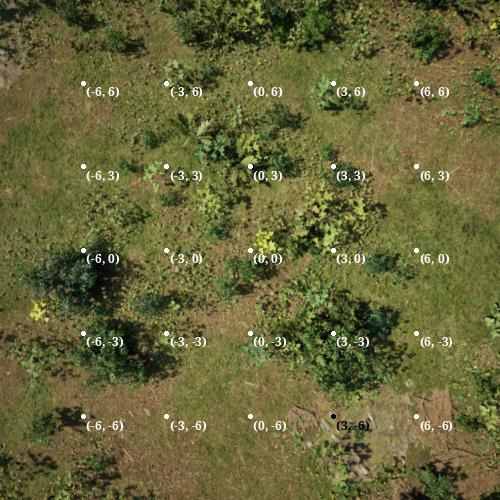
\includegraphics[width=0.5\linewidth]{images/Sonnet-ForestNew/21_r0__7.jpg}
    \end{center}
    
\respeaks: Your current altitude is 9 meters above ground level.
\gptspeaks: \( < \)Reasoning\( > \)I need to rethink my strategy. We only have one move left after this one, and I haven't located the fire yet. Looking back at the first image, the fire was in the southeastern quadrant, but I might have moved in the wrong direction. Let me try moving back towards where we started and then southeast.\( < \)/Reasoning\( > \)
\( < \)Action\( > \)(0, -6, 0)\( < \)/Action\( > \)
\respeaks: Image 9:
\StageDir{\re{} presents \gpt{} with a relevant image}

    \begin{center}
    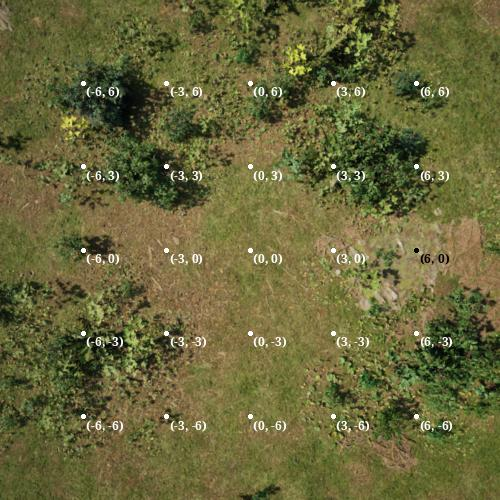
\includegraphics[width=0.5\linewidth]{images/Sonnet-ForestNew/21_r0__8.jpg}
    \end{center}
    
\respeaks: Your current altitude is 9 meters above ground level.
\gptspeaks: \( < \)Reasoning\( > \)Unfortunately, I have not been successful in locating the fire. While I maintained the correct altitude of 9 meters throughout the search, my navigation strategy was not effective in reaching the fire location that we initially saw in the southeastern portion of the first image. I've used all 9 allowed moves without successfully centering on the fire.\( < \)/Reasoning\( > \)
\( < \)Action\( > \)(0, -6, 0)\( < \)/Action\( > \)
\respeaks: Image 10:
\StageDir{\re{} presents \gpt{} with a relevant image}

    \begin{center}
    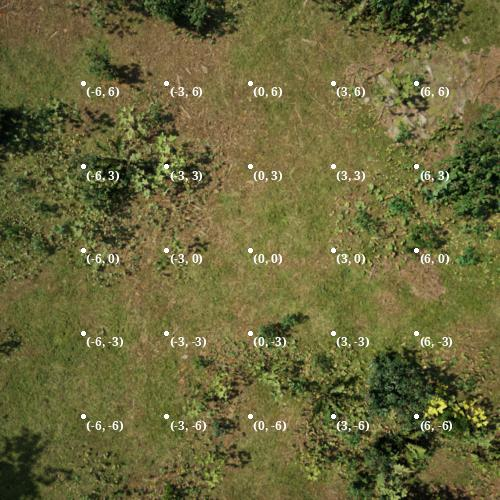
\includegraphics[width=0.5\linewidth]{images/Sonnet-ForestNew/21_r0__9.jpg}
    \end{center}
    
\respeaks: Your current altitude is 9 meters above ground level.
\gptspeaks: \( < \)Reasoning\( > \)I have now used all available moves and was not successful in my mission. While I maintained the correct altitude of 9 meters, which would have been appropriate for identifying the fire, my search pattern was ineffective. I should have made larger initial movements towards the southeastern direction where we first spotted the fire, while still staying within the safe visible boundaries. This would have been a better strategy than the smaller incremental movements I chose to make.\( < \)/Reasoning\( > \)
\end{drama}
\subsubsection{Example}

    \begin{itemize}[noitemsep,topsep=0pt]
      \item Starting position: (18.0, -20.0, 71.0)
      \item End position: (27.0, -1.0, 7.0) 
      \item Euclidean distance from the object: 27.910571473905726
      \item Object can be seen: False
      \item Success: False
      \item Object type: a trash pile
      
    \end{itemize}
    

    \begin{center}
    \includegraphics[width=0.7\linewidth]{images/Sonnet-ForestNew/22_r0_.pdf}
    \end{center}
    

    \begin{center}
    \includegraphics[width=0.7\linewidth]{images/Sonnet-ForestNew/22_r0__sit_awareness.pdf}
    \end{center}
    

    \begin{drama}
    \Character{Benchmark}{re}
    \Character{Claude 3.5 Sonnet}{gpt}
    
\respeaks: \( < \)Context\( > \)
    You are in command of a UAV, tasked with finding a trash pile.
\( < \)/Context\( > \) \texttt{(REST OF THE PROMPT)}
\respeaks: Image 1:
\StageDir{\re{} presents \gpt{} with a relevant image}

    \begin{center}
    
\includegraphics[width=0.5\linewidth]{images/Sonnet-ForestNew/22_r0__0.jpg}
    \end{center}
    
\respeaks: Your current altitude is 70 meters above ground level.
\gptspeaks: \( < \)Reasoning\( > \)
I need to start searching for the trash pile systematically. From this altitude (70m), it's difficult to spot small details clearly. I notice some variations in the terrain, but I need to get lower to better identify potential targets. I'll move to a central position and decrease altitude significantly to get a better view of the area.

I'll move towards coordinates (0, 0) which is the center of the grid, and simultaneously decrease altitude by 40 meters to get a better view while maintaining enough height to continue searching if needed.
\( < \)/Reasoning\( > \)
\( < \)Action\( > \)(0, 0, -40)\( < \)/Action\( > \)
\respeaks: Image 2:
\StageDir{\re{} presents \gpt{} with a relevant image}

    \begin{center}
    
\includegraphics[width=0.5\linewidth]{images/Sonnet-ForestNew/22_r0__1.jpg}
    \end{center}
    
\respeaks: Your current altitude is 29 meters above ground level.
\gptspeaks: \( < \)Reasoning\( > \)
From this lower altitude (29m), I can see more details but I still don't clearly spot the trash pile. I notice some variations in the terrain and coloring in the southeast quadrant of the visible area. I'll move towards that direction (10, -10) and lower the altitude a bit more to get an even better view of that area.
\( < \)/Reasoning\( > \)
\( < \)Action\( > \)(10, -10, -15)\( < \)/Action\( > \)
\respeaks: Image 3:
\StageDir{\re{} presents \gpt{} with a relevant image}

    \begin{center}
    
\includegraphics[width=0.5\linewidth]{images/Sonnet-ForestNew/22_r0__2.jpg}
    \end{center}
    
\respeaks: Your current altitude is 13 meters above ground level.
\gptspeaks: \( < \)Reasoning\( > \)
At this altitude (13m), I'm quite close to the vegetation, but I still need to continue my search. I can see mostly leaves and foliage in this area, but no trash pile. I'll move slightly east and south where there seems to be a bit more open space between the vegetation, and maintain this altitude to get a good view of that area.
\( < \)/Reasoning\( > \)
\( < \)Action\( > \)(4, -4, 0)\( < \)/Action\( > \)
\respeaks: Image 4:
\StageDir{\re{} presents \gpt{} with a relevant image}

    \begin{center}
    
\includegraphics[width=0.5\linewidth]{images/Sonnet-ForestNew/22_r0__3.jpg}
    \end{center}
    
\respeaks: Your current altitude is 12 meters above ground level.
\gptspeaks: \( < \)Reasoning\( > \)
I can now see what appears to be some debris or trash (dark objects) near the center of the image. Since I need to be below 10 meters and centered on the object, I'll move to position (0, 0) and descend a few more meters to get below the 10-meter requirement while staying centered over what appears to be the trash pile.
\( < \)/Reasoning\( > \)
\( < \)Action\( > \)(0, 0, -4)\( < \)/Action\( > \)
\respeaks: Image 5:
\StageDir{\re{} presents \gpt{} with a relevant image}

    \begin{center}
    
\includegraphics[width=0.5\linewidth]{images/Sonnet-ForestNew/22_r0__4.jpg}
    \end{center}
    
\respeaks: Your current altitude is 7 meters above ground level.
\gptspeaks: FOUND

\( < \)Reasoning\( > \)
I am now perfectly positioned at 7 meters altitude, which is below the required 10 meters, and I am centered over what appears to be a collection of debris/trash (dark objects scattered on the ground). The trash pile is clearly visible in my field of view and I am centered on it at coordinates (0,0).
\( < \)/Reasoning\( > \)
\end{drama}
